\documentclass{standalone}
\usepackage{tikz}
\usetikzlibrary{patterns, positioning}
\usepackage[sfdefault]{ClearSans} %% option 'sfdefault' activates Clear Sans as the default text font
\usepackage[T1]{fontenc}

\begin{document}
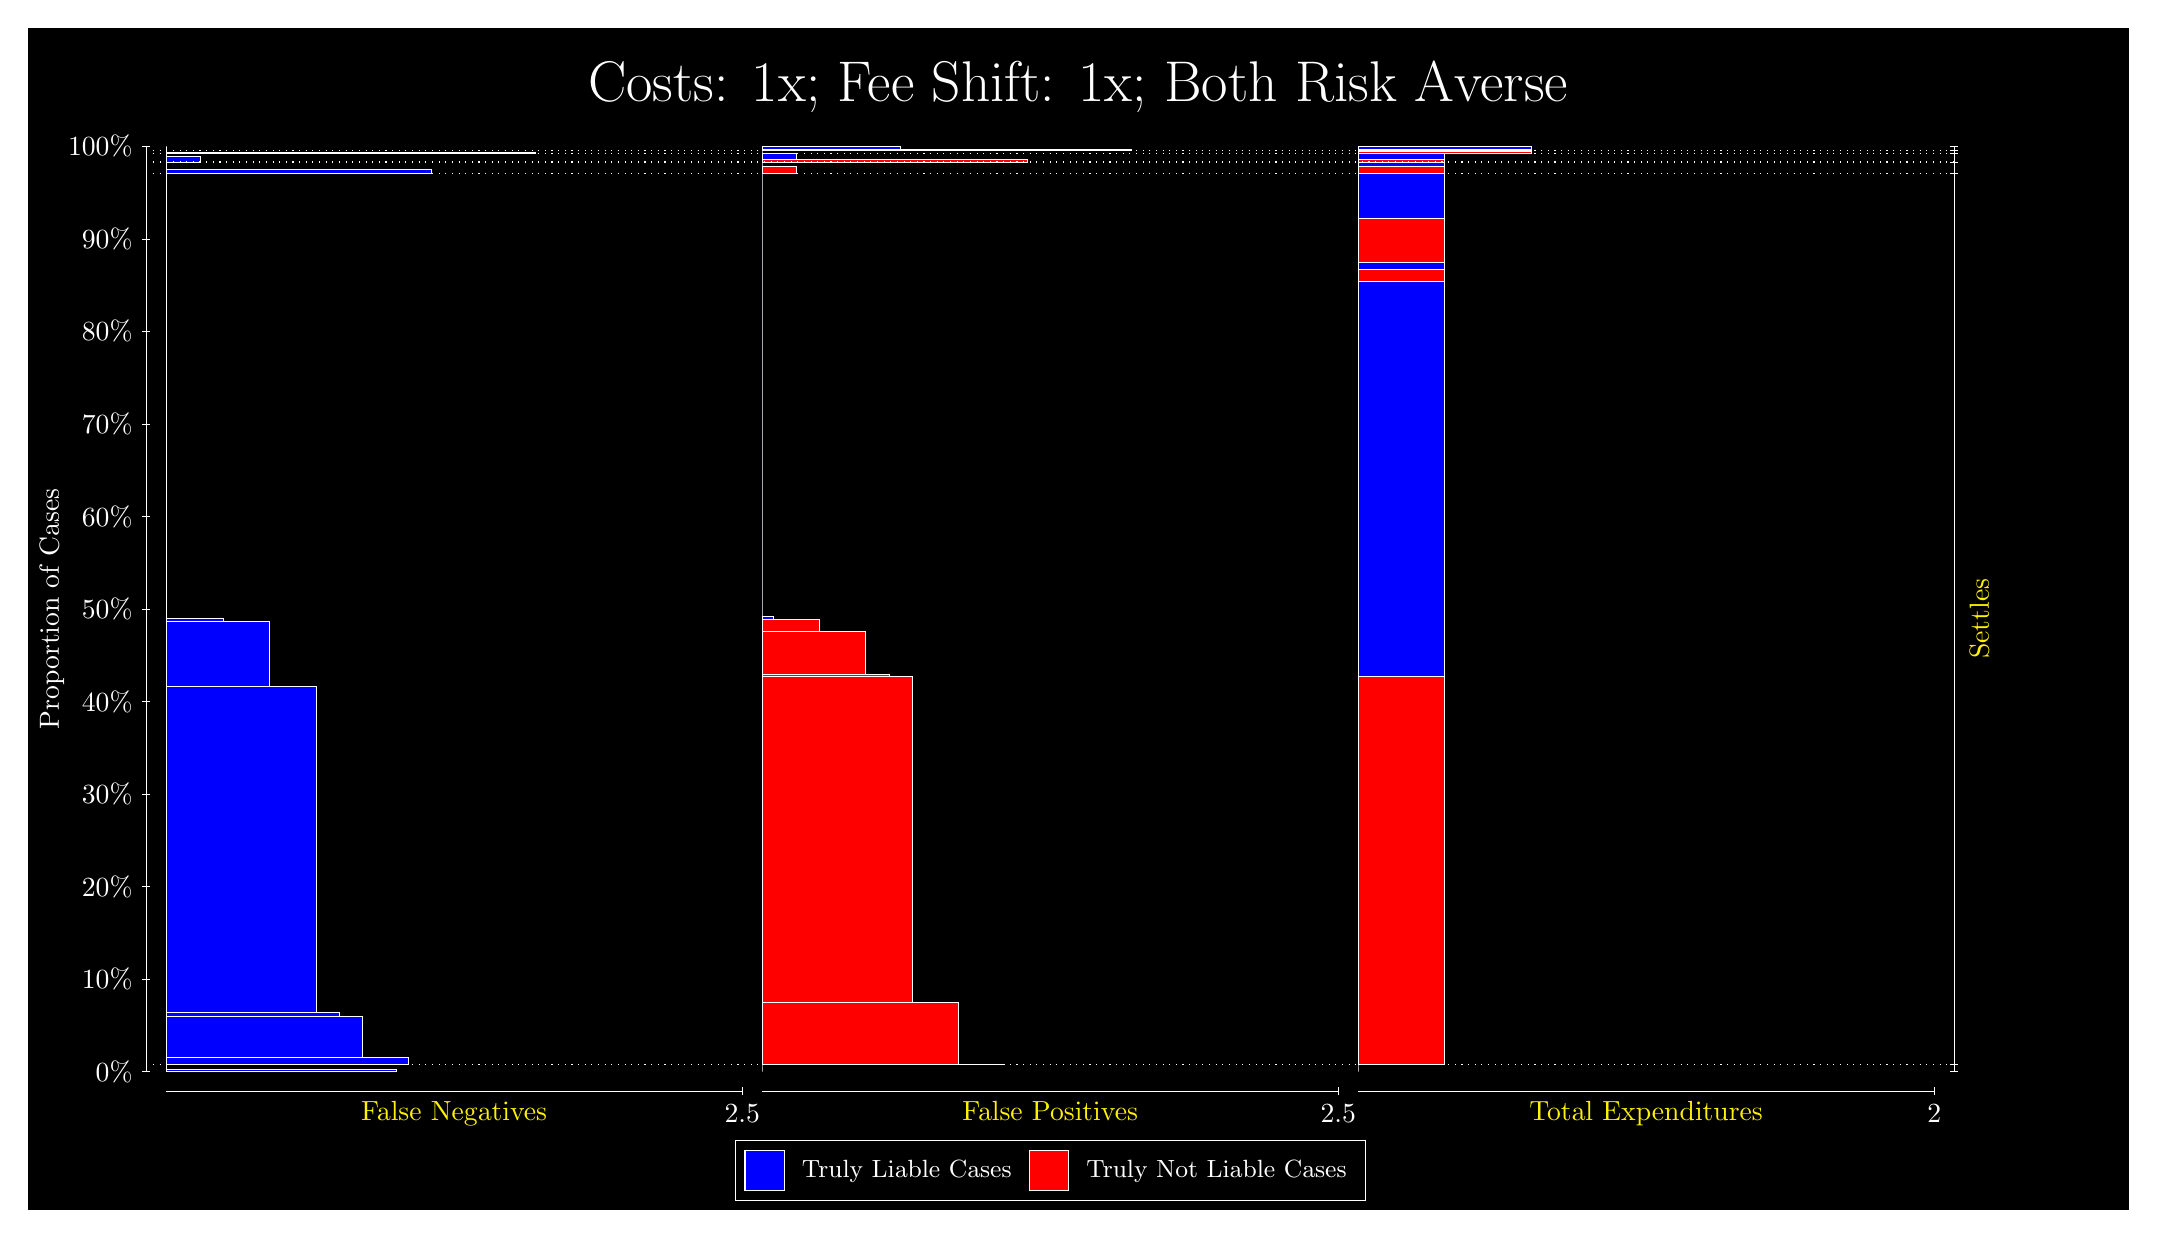
\begin{tikzpicture}
\draw[fill=black] (0,0) rectangle (26.667,15);
\draw[text=white] (0,13.5) rectangle (26.667,15) node[midway] {\huge Costs: 1x; Fee Shift: 1x; Both Risk Averse};
\draw[white, very thin] (1.5,1.75) -- (1.5,13.5);
\node[rotate=90, text=white, anchor=center] at (0.3, 7.625) {Proportion of Cases};
\draw[white, very thin] (1.45,1.75) -- (1.55,1.75);
\node[text=white, anchor=east] at (1.45, 1.75) {0\%};
\draw[white, very thin] (1.45,2.925) -- (1.55,2.925);
\node[text=white, anchor=east] at (1.45, 2.925) {10\%};
\draw[white, very thin] (1.45,4.1) -- (1.55,4.1);
\node[text=white, anchor=east] at (1.45, 4.1) {20\%};
\draw[white, very thin] (1.45,5.275) -- (1.55,5.275);
\node[text=white, anchor=east] at (1.45, 5.275) {30\%};
\draw[white, very thin] (1.45,6.45) -- (1.55,6.45);
\node[text=white, anchor=east] at (1.45, 6.45) {40\%};
\draw[white, very thin] (1.45,7.625) -- (1.55,7.625);
\node[text=white, anchor=east] at (1.45, 7.625) {50\%};
\draw[white, very thin] (1.45,8.8) -- (1.55,8.8);
\node[text=white, anchor=east] at (1.45, 8.8) {60\%};
\draw[white, very thin] (1.45,9.975) -- (1.55,9.975);
\node[text=white, anchor=east] at (1.45, 9.975) {70\%};
\draw[white, very thin] (1.45,11.15) -- (1.55,11.15);
\node[text=white, anchor=east] at (1.45, 11.15) {80\%};
\draw[white, very thin] (1.45,12.325) -- (1.55,12.325);
\node[text=white, anchor=east] at (1.45, 12.325) {90\%};
\draw[white, very thin] (1.45,13.5) -- (1.55,13.5);
\node[text=white, anchor=east] at (1.45, 13.5) {100\%};

\draw[white, very thin] (24.457,1.75) -- (24.457,13.5);
\draw[white, very thin] (24.407,1.75) -- (24.507,1.75);
\node[anchor=west] at (24.407, 1.75) {};
\draw[white, very thin] (24.407,1.8393) -- (24.507,1.8393);
\node[anchor=west] at (24.407, 1.8393) {};
\draw[white, very thin] (24.407,13.16) -- (24.507,13.16);
\node[anchor=west] at (24.407, 13.16) {};
\draw[white, very thin] (24.407,13.301) -- (24.507,13.301);
\node[anchor=west] at (24.407, 13.301) {};
\draw[white, very thin] (24.407,13.408) -- (24.507,13.408);
\node[anchor=west] at (24.407, 13.408) {};
\draw[white, very thin] (24.407,13.452) -- (24.507,13.452);
\node[anchor=west] at (24.407, 13.452) {};
\draw[white, very thin] (24.407,13.5) -- (24.507,13.5);
\node[anchor=west] at (24.407, 13.5) {};

\draw[white, very thin, fill=blue] (1.75,1.75) rectangle (4.6775,1.7745);
\draw[white, very thin, fill=red] (1.75,1.7745) rectangle (1.75,1.8393);
\draw[white, very thin, fill=blue] (1.75,1.8393) rectangle (4.8239,1.9295);
\draw[white, very thin, fill=blue] (1.75,1.9295) rectangle (4.2384,2.4519);
\draw[white, very thin, fill=blue] (1.75,2.4519) rectangle (3.9457,2.5013);
\draw[white, very thin, fill=blue] (1.75,2.5013) rectangle (3.6529,6.6411);
\draw[white, very thin, fill=blue] (1.75,6.6411) rectangle (3.0674,7.4722);
\draw[white, very thin, fill=blue] (1.75,7.4722) rectangle (2.4819,7.5085);
\draw[white, very thin, fill=red] (1.75,7.5085) rectangle (1.75,13.16);
\draw[white, very thin, fill=blue] (1.75,13.16) rectangle (5.1167,13.214);
\draw[white, very thin, fill=red] (1.75,13.214) rectangle (1.75,13.301);
\draw[white, very thin, fill=blue] (1.75,13.301) rectangle (2.1891,13.377);
\draw[white, very thin, fill=red] (1.75,13.377) rectangle (1.75,13.408);
\draw[white, very thin, fill=blue] (1.75,13.408) rectangle (6.4341,13.426);
\draw[white, very thin, fill=red] (1.75,13.426) rectangle (1.75,13.452);
\draw[white, very thin, fill=red] (1.75,13.452) rectangle (1.75,13.468);
\draw[white, very thin, fill=blue] (1.75,13.468) rectangle (1.75,13.5);
\draw[white, very thin, fill=red] (9.3189,1.75) rectangle (9.3189,1.8148);
\draw[white, very thin, fill=blue] (9.3189,1.8148) rectangle (9.3189,1.8393);
\draw[white, very thin, fill=red] (9.3189,1.8393) rectangle (12.393,1.8474);
\draw[white, very thin, fill=red] (9.3189,1.8474) rectangle (11.807,2.6352);
\draw[white, very thin, fill=red] (9.3189,2.6352) rectangle (11.222,6.775);
\draw[white, very thin, fill=red] (9.3189,6.775) rectangle (10.929,6.8004);
\draw[white, very thin, fill=red] (9.3189,6.8004) rectangle (10.636,7.3349);
\draw[white, very thin, fill=red] (9.3189,7.3349) rectangle (10.051,7.4909);
\draw[white, very thin, fill=blue] (9.3189,7.4909) rectangle (9.4652,7.5272);
\draw[white, very thin, fill=blue] (9.3189,7.5272) rectangle (9.3189,13.16);
\draw[white, very thin, fill=red] (9.3189,13.16) rectangle (9.758,13.246);
\draw[white, very thin, fill=blue] (9.3189,13.246) rectangle (9.3189,13.301);
\draw[white, very thin, fill=red] (9.3189,13.301) rectangle (12.686,13.331);
\draw[white, very thin, fill=blue] (9.3189,13.331) rectangle (9.758,13.408);
\draw[white, very thin, fill=red] (9.3189,13.408) rectangle (9.3189,13.433);
\draw[white, very thin, fill=blue] (9.3189,13.433) rectangle (9.3189,13.452);
\draw[white, very thin, fill=red] (9.3189,13.452) rectangle (14.003,13.468);
\draw[white, very thin, fill=blue] (9.3189,13.468) rectangle (11.075,13.5);
\draw[white, very thin, fill=red] (16.888,1.75) rectangle (16.888,1.8148);
\draw[white, very thin, fill=blue] (16.888,1.8148) rectangle (16.888,1.8393);
\draw[white, very thin, fill=red] (16.888,1.8393) rectangle (17.986,6.775);
\draw[white, very thin, fill=blue] (16.888,6.775) rectangle (17.986,11.782);
\draw[white, very thin, fill=red] (16.888,11.782) rectangle (17.986,11.938);
\draw[white, very thin, fill=blue] (16.888,11.938) rectangle (17.986,12.028);
\draw[white, very thin, fill=red] (16.888,12.028) rectangle (17.986,12.588);
\draw[white, very thin, fill=blue] (16.888,12.588) rectangle (17.986,13.16);
\draw[white, very thin, fill=red] (16.888,13.16) rectangle (17.986,13.246);
\draw[white, very thin, fill=blue] (16.888,13.246) rectangle (17.986,13.301);
\draw[white, very thin, fill=red] (16.888,13.301) rectangle (17.986,13.331);
\draw[white, very thin, fill=blue] (16.888,13.331) rectangle (17.986,13.408);
\draw[white, very thin, fill=red] (16.888,13.408) rectangle (19.083,13.433);
\draw[white, very thin, fill=blue] (16.888,13.433) rectangle (19.083,13.452);
\draw[white, very thin, fill=red] (16.888,13.452) rectangle (19.083,13.468);
\draw[white, very thin, fill=blue] (16.888,13.468) rectangle (19.083,13.5);
\draw[white, dotted] (1.5,1.8393) -- (24.457,1.8393);
\draw[white, dotted] (1.5,13.16) -- (24.457,13.16);
\draw[white, dotted] (1.5,13.301) -- (24.457,13.301);
\draw[white, dotted] (1.5,13.408) -- (24.457,13.408);
\draw[white, dotted] (1.5,13.452) -- (24.457,13.452);
\draw[white, very thin] (1.75,1.5) -- (9.0689,1.5);
\node[text=yellow, anchor=north] at (5.4094, 1.5) {False Negatives};
\draw[white, very thin] (9.0689,1.45) -- (9.0689,1.55);
\node[text=white, anchor=north] at (9.0689, 1.45) {2.5};

\draw[white, very thin] (9.3189,1.5) -- (16.638,1.5);
\node[text=yellow, anchor=north] at (12.978, 1.5) {False Positives};
\draw[white, very thin] (16.638,1.45) -- (16.638,1.55);
\node[text=white, anchor=north] at (16.638, 1.45) {2.5};

\draw[white, very thin] (16.888,1.5) -- (24.207,1.5);
\node[text=yellow, anchor=north] at (20.547, 1.5) {Total Expenditures};
\draw[white, very thin] (24.207,1.45) -- (24.207,1.55);
\node[text=white, anchor=north] at (24.207, 1.45) {2};


\node[text=yellow, centered, rotate=90] at (24.777, 7.4997) {Settles};





\draw (12.978300999999998,1.5) node[draw=none] (baseCoordinate) {};
\begin{scope}[align=center]
        \matrix[scale=0.5, draw=white, below=0.5cm of baseCoordinate, nodes={draw}, column sep=0.1cm]{
            \node[rectangle, draw, minimum width=0.5cm, minimum height=0.5cm, fill=blue] {}; &
            \node[draw=none, font=\small, text=white] (B) {Truly Liable Cases}; &
            \node[rectangle, draw, minimum width=0.5cm, minimum height=0.5cm, fill=red] {}; &
            \node[draw=none, font=\small, text=white] (B) {Truly Not Liable Cases}; \\
            };
\end{scope}

\end{tikzpicture}
\end{document}